\chapter{Data basis}
\label{chap:data_basis}

The previous chapter mentioned parameters affecting hydroelectricity production. In this chapter, the data sets available for this work will be described and analyzed. This include power plants data registers and production data, as well as runoff data sets. 

\section{Hydroelectricity}
\label{sec:db_hydroelec}
In order to simulate the hydroelectricity production of a region, a register of all existing power plants is needed. The simulated hydroelectricity production should then be compared to real production data, in order to validate the model. This process can only be consistent if the actual production data comes from the same plants listed in the power plants register. This section presents the available data sets for existing plants and production, and shows the significant discrepancies between them. 

\subsection{Open Energy Database}
\label{sub:hpp_reg}
This work, as well as the project open\_FRED, is linked to the OpenEnergy Platform, developed within the open\_eGo project. The OpenEnergy Platform, through the OpenEnergy Database, provides necessary tools for transparent and collaborative energy system modeling \cite{oedb}, such as grid data, power plants register, geography data or weather data. The power plant register was extracted from the Open Power System Data (OPSD) and has 7491 entries for run-of-the-river hydropower plants and 5 entries for reservoir plants in Germany. The run-of-the-river entries contain, among others, the following information :
\begin{itemize}
\itemsep-0.5em 
 \item Company operating the plant and network operator information
 \item Adress and state
 \item Startup, retrofit and shutdown years
 \item Electrical capacity [\unit{MW}]
 \item Position (latitude, longitude, and GIS geometry)
\end{itemize}

Figure \ref{oedb_capa} shows the repartition of the capacity of OPSD run-of-the-river and reservoir plants. This is consistent with the Umweltbundesamt numbers of 6500 to 7500 hydropower plants excluding pumped hydro, among which 406 with a nominal power above \unit[1]{MW} \cite{uba_wasserkraft}. The OPSD also has entries for pumped storage plants, listed in Tab. \ref{oedb_pump}.

\begin{figure}[H]
\centering
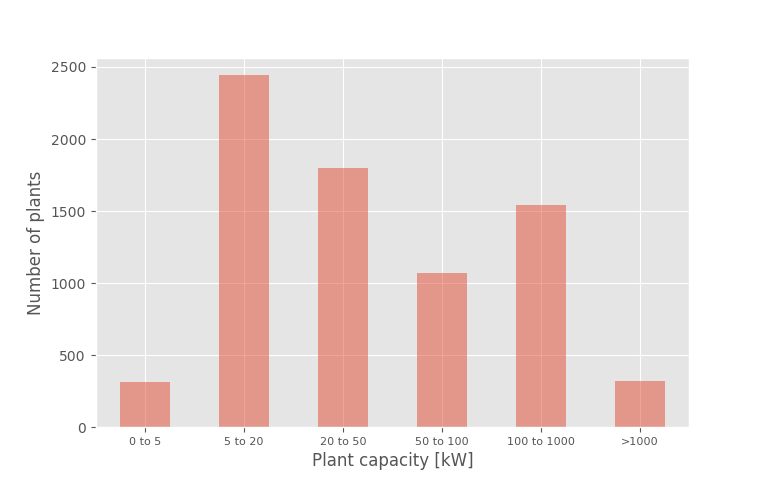
\includegraphics[width=10cm]{oedb_capa.png}
\caption[Repartition of the capacity of run-of-the-river and reservoir plants in the Open Power System Data]{Repartition of the capacity of run-of-the-river plants plants in the Open Power System Data}
\label{oedb_capa}
\end{figure}

\begin{table} [H]
\footnotesize
  \centering
  \caption[Number of pumped storage plants and installed capacity per federal state]{Number of pumped storage plants and installed capacity per federal state \cite{oedb}}
  \label{oedb_pump}
  \begin{tabular}{|c|cc| }
  \hline
  \textbf{State} & Number 	& 	Capacity [\unit{MW}] 	\\
  \hline
  SH	&	3	&	119.1	\\
  NI	&	1	&	220	\\
  NRW	&	2	&	291	\\
  HE	&	2	&	623	\\
  BW	&	7	&	1873	\\	
  BY	&	7	&	587	\\
  SN	&	8	&	1085	\\
  ST	&	2	&	79.7	\\
  TH	&	16	&	1509.4	\\
  \hline
  \end{tabular}
\end{table}

\subsection{Comparison with the Agentur für Erneuerbare Energie data}
\label{sub:prod_data}

A simulation based on the OPSD register should be compared with real production data, to assess the precision of the model.\newline The hydroelectricity production of Germany is calculated by the Bundesverband der Energie- und Wasserwirtschaft (BDEW), a federal organisation of companies in the sector of water and energy, and published by the Agentur für Erneuerbare Energien (AEE). The AEE provides data about the installed capacity, electricity generation over the year, and number of hydropower plants for each federal state from 2001 to 2014 \cite{aee}. This data contains run-of-the-river and reservoir plants, as well as pumped storage power plants with natural inflow for which only the production from natural inflow is accounted for. There is therefore no consistent way of comparing it with the OPSD data because the OPSD does not state which part of the capacity of pumped hydro plants uses natural inflow. \newline
Table \ref{oedb_aee_diff} lists the number of plants and installed capacity per federal state from the OPSD (run-of-the-river and reservoirs) and the AEE, as well as the relative difference for each state, with the AEE data as reference. It shows that even in states with no pumped storage facilities, such as Rhineland-Palatinate, these two sources give very different values for the numbers of plants and installed capacities. \newline
The relative difference is shown on figures \ref{map_diff_num} and \ref{map_diff_pow}, which respectively display the differences in the number of plants and in the installed capacity. The analysis of these two maps and of Tab. \ref{oedb_aee_diff} shows that the OPSD and AEE data sets seem to be consistent in three federal states : Thuringia, Saxony-Anhalt and Mecklenburg-Vorpommern (Berlin and Bremen being excluded due to the near absence of hydropower). The discrepancies in other federal states can be explained by different reasons. First, the data of the the AEE are based on run-of-the-river plants, reservoir plants and natural inflow in pumped storage plants, while the data from the OPSD shown here only account for run-of-the-river and reservoir plants (the pumped hydro plants having been excluded due to the lack of information on the presence of natural inflow). Moreover, the OPSD register of reservoir plants, with its five entries, is clearly incomplete. This is why both the number of plants and the installed capacity are greater in the AEE data for most states. Second, the pumped storage and reservoir plants tend to have a bigger capacity than most run-of-the-river plants, which explains that the difference in installed capacity is not proportional to the difference in number of plants. Finally, rivers often mark boundaries between states and countries, and some hydropower plant are operated by two countries or inject electricity into the grid of a neighboring country. It is possible that the AEE and the OPSD do not count the installed capacity in the same manner in this situation.

\begin{table}[H]
\footnotesize 
 \centering
 \caption[Number of hydropower plants and installed capacity per federal state]{Number of hydropower plants and installed capacity per federal state}
 \label{oedb_aee_diff}
 \begin{tabular}{|c|cc|cc| cc|}
  \cline{2-7}
  \multicolumn{0}{c|}{} &\multicolumn{2}{c}{\textbf{OPSD \cite{oedb}}}&\multicolumn{2}{|c|}{\textbf{AEE \cite{aee}}}&\multicolumn{2}{c|}{\textbf{Difference}} \\
  \hline
  \textbf{State} & Number 	& 	Capacity [\unit{MW}] 	&	Number 	& 	Capacity [\unit{MW}] 	&	Number [\unit{\%}] 	&	Capacity [\unit{\%}] \\
  \hline
  SH	&	29	&	8.1		&	24	&	5		&	20.8		&	62.8	\\
  HH	&	1	&	0.11		&	1	&	0.1		&	0		&	10	\\
  NI	&	258	&	56.3		&	257	&	70		&	0.4		&	-19	\\
  HB	&	1	&	10		&	1	&	10		&	0		&	0	\\
  NRW	&	438	&	152.8		&	409	&	202		&	7.1		&	-24.3	\\
  HE	&	465	&	91.9		&	482	&	82		&	-3.5		&	12.1	\\
  RLP	&	217	&	40.8		&	199	&	218		&	9		&	-81.3	\\
  BW	&	1741	&	464.5		&	1485	&	960		&	17		&	-51.6	\\	
  BY	&	3659	&	835.7		&	3578	&	2661		&	2.3		&	-68.6	\\
  SL	&	26	&	11.1		&	26	&	24		&	0		&	-53.6	\\
  B	&	0	&	0		&	0	&	0		&	0		&	0	\\
  BB	&	42	&	5.3		&	38	&	6		&	10.5		&	-11.8	\\
  MV	&	25	&	3		&	24	&	3		&	4.2		&	-0.1	\\
  SN	&	322	&	134.4		&	330	&	99		&	-2.4		&	35.8	\\
  ST	&	57	&	26		&	52	&	26		&	9.6		&	0.2	\\
  TH	&	205	&	32.6		&	198	&	32		&	3		&	2	\\
  \hline
 \end{tabular} 
\end{table}


\begin{figure}[H]
\centering
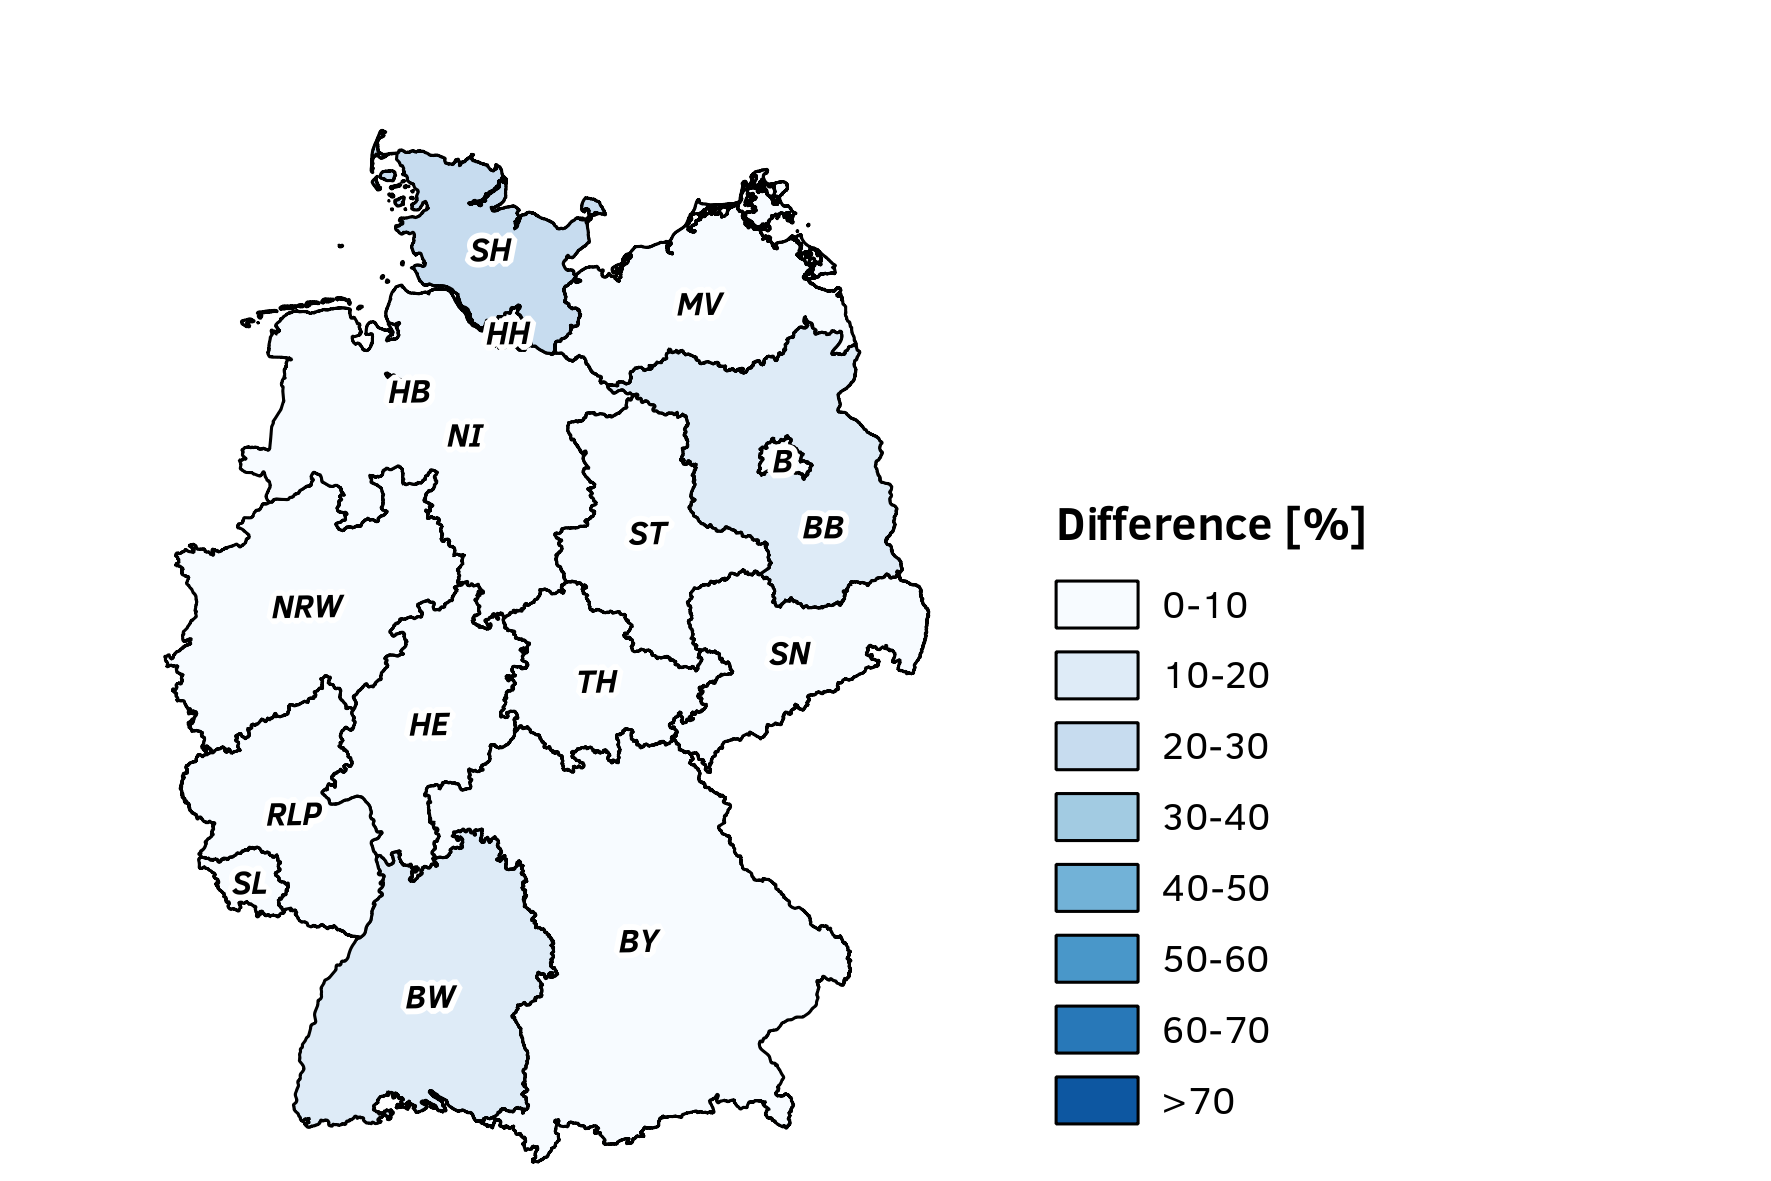
\includegraphics[width=13cm]{map_diff_num.png}
\caption[Absolute difference in the number of plants between OPSD and AEE]{Absolute difference in the number of plants between OPSD and AEE}
\label{map_diff_num}
\end{figure}


\begin{figure}[H]
\centering
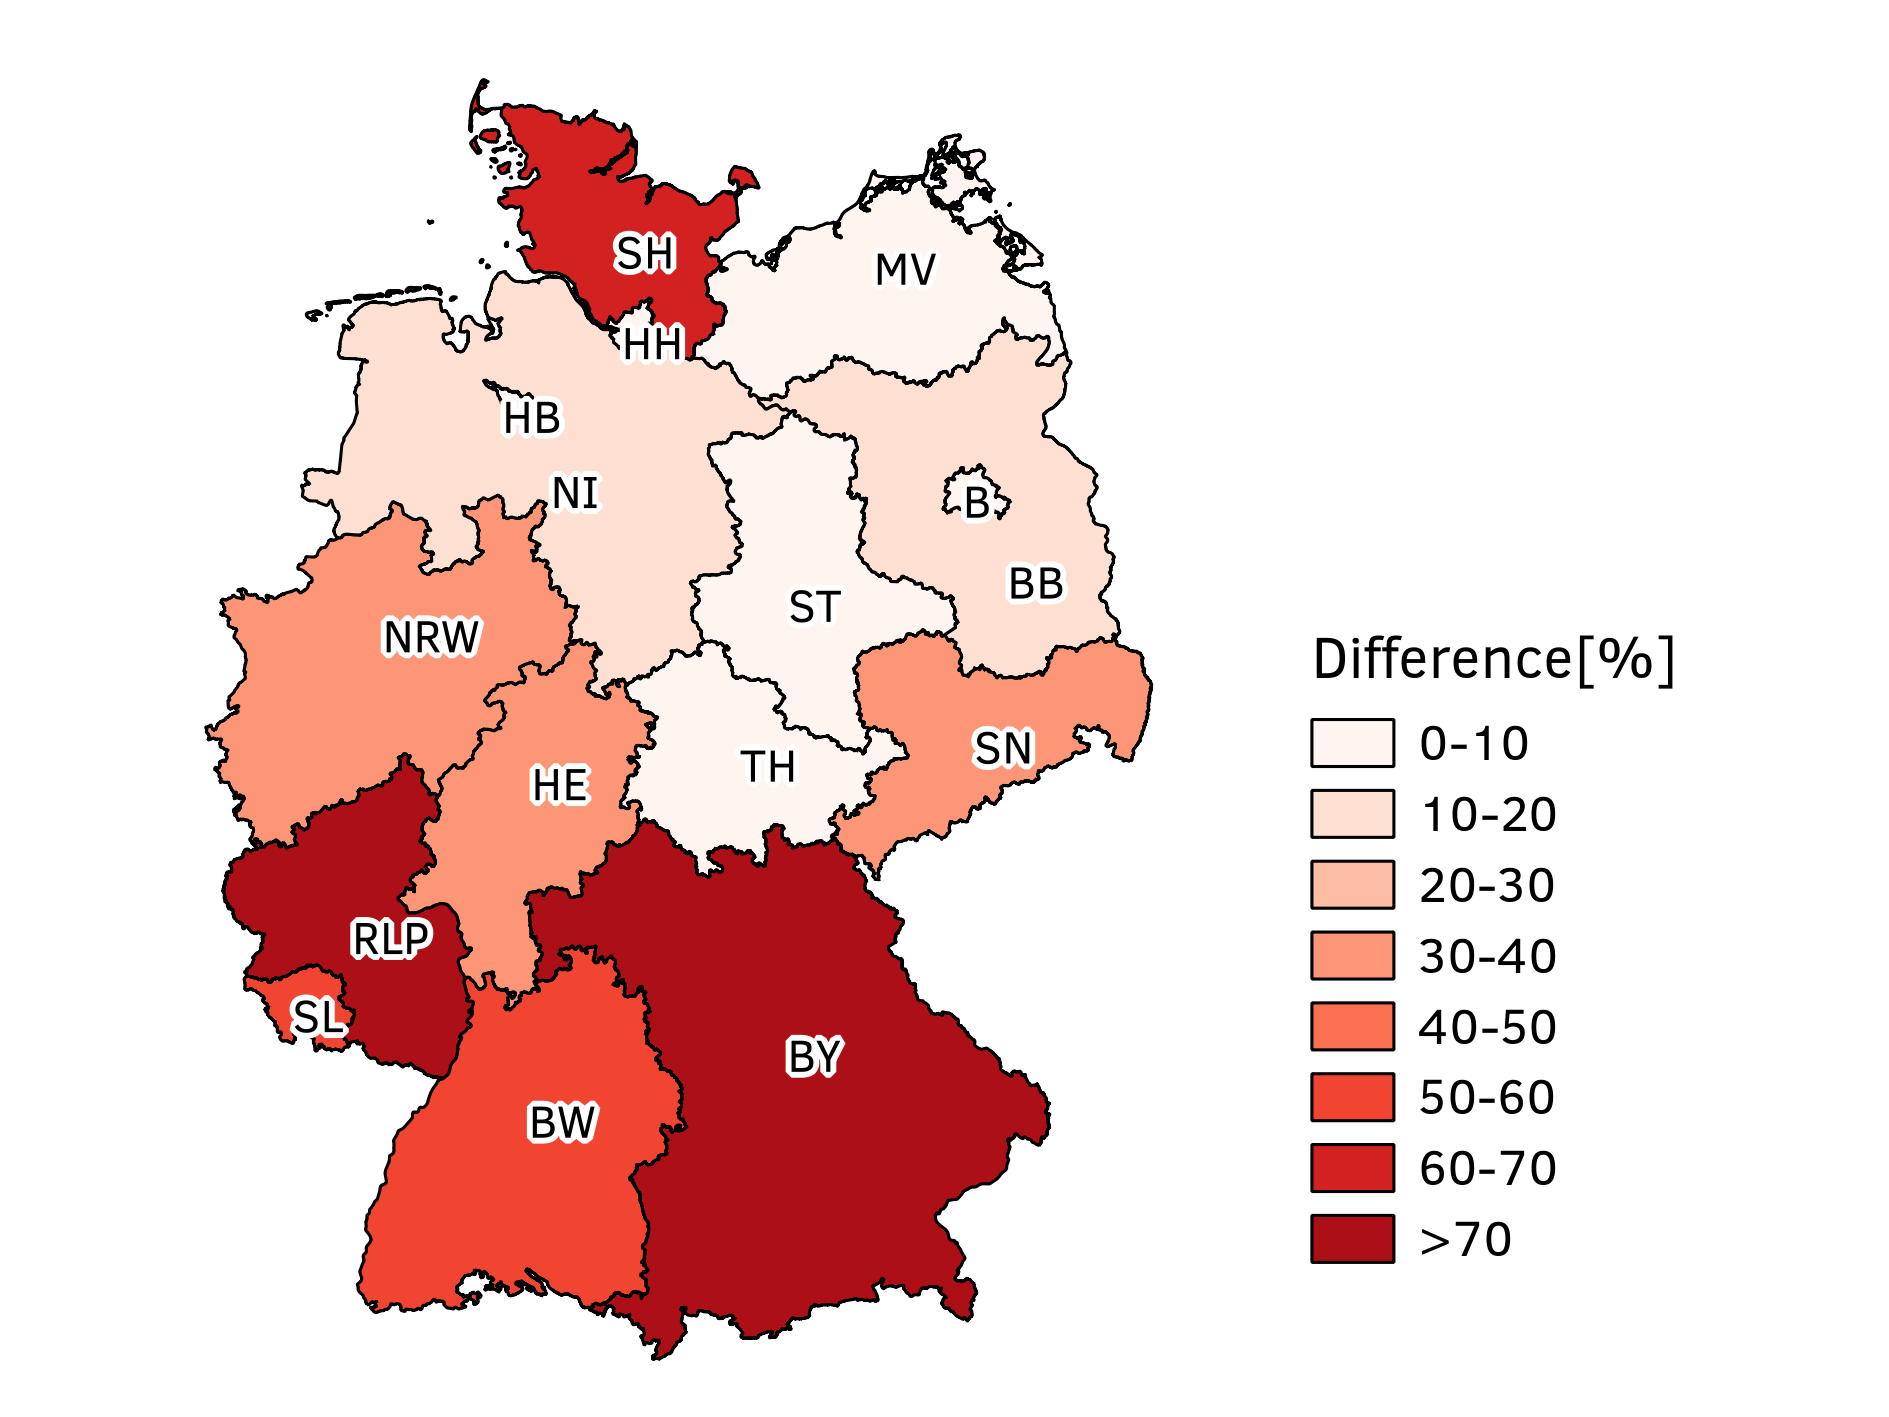
\includegraphics[width=13cm]{map_diff_pow.png}
\caption[Absolute difference in the installed capacity between OPSD and AEE]{Absolute difference in the installed capacity between OPSD and AEE}
\label{map_diff_pow}
\end{figure}


\subsection{Future data set}

The german Bundesnetzagentur is developing a register of every energy production facility in Germany, called ``Marktstammdatenregister''. This register should give a complete overview of the power plants in Germany, sorted by energy carrier and type of plant (reservoir, run-of-the-river, pumped hydro...), and listing the location and nominal power, as well as the presence or not of a restriction of the usable water flow due to a fish ladder or fish protection system for instance \cite{MaStR}. \newline
When published, it will be uploaded in the OEDB and will provide a more consistent data set of existing plants.

\section{Runoff data - measured}

\label{sec:meas_runoff}

In order to study rivers, 

Water levels and water flows of the main rivers are regularly measured and documented by several organizations, in order to keep track of the history of the waterways and to anticipate potential floods. Measurement stations have been installed and monitored for decades, dating back as far as 1816 for Germany, and the time series are stored in databases. There are different ways to measure the water flow, such as propeller gauges, ultrasonic flow meter, or acoustic current profilers. In Germany there are around 4300 stations measuring water flow or water level, operated by different stakeholders \cite{bafg_hyd}.  The German Federal Institute of Hydrology (Bundesanstalt für Gewässerkunde – BfG) is a supreme federal agency within the portfolio of the Federal Ministry of Transport and Digital Infrastructure. As such it is the federal government's scientific institution for research, assessments, and consulting in the fields of hydrology, uses, quality and conservation of waters and ecology \cite{bafg}. The BfG gathers data about water levels and water flows since its founding in 1949 and publishes it every year in the ``Deutsches Gewässerkundliches Jahrbuch'' (DGJ). The BfG also operates the HYDABA database, in which times series for water flow and water level are stored, going back to 1816 for daily values and 1981 for hourly values. This database gathers water levels from around 600 gauges and water flows from around 250 stations, operated by the Federal Waterways and Shipping Administration (WSV). The data from the HYDABA database can be provided to, among others, universities, public administrations, engineering or insurance companies \cite{bafg_hyd}. \newline
The WSV, through its service Pegelonline, publishes raw values of water levels from its gauge stations in Germany over the previous 30 days. Some of the stations also measure water flows \cite{pegelonline}. The locations of the gauges are shown on Fig. \ref{pegelonline}.

\begin{figure}[H]
\centering
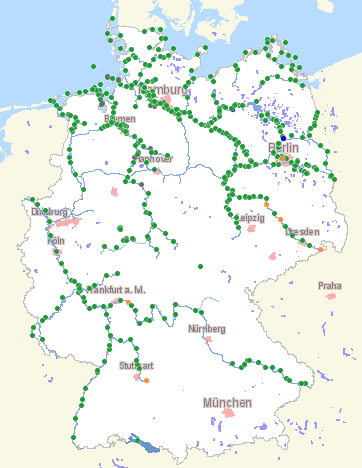
\includegraphics[width=8cm]{pegelonline.png}
\caption[Locations of the gauge stations]{Locations of the gauge stations \cite{pegelonline}}
\label{pegelonline}
\end{figure}

Another source for runoff data is the Global Runoff Data Center (GRDC, 56068 Koblenz, Germany) which operates, on a non-profit basis, a world-wide database of measured runoffs. The GRDC can transfer its data on demand and under certain conditions (according to its policy guidelines for the dissemination of data).\newline

Other countries have similar databases for measured river data. In France, the ``Banque Hydro'' is run by the SCHAPI (Service Central d'Hydrométéorologie et d'Appui à la Prévision des Inondations), a section of the french Ministry of Ecology, Sustainable Development and Energy, and gathers and publishes data from around 5000 gauge stations.

\section{Runoff data - modeled}

\label{sec:mod_runoff}
Modeling runoff is a difficult task, as the model has to assess the interactions between river sources, relief, rainfall, local soil and vegetation type, as well as anthropogenic use. This can be done using GIS \cite{bayazit}, by assigning each cell with the precedent parameters. The water input in each cell (rainfall, water sources and runoff from other cells) is converted in runoff from the cell by subtracting the water lost by infiltration, evapotranspiration, or anthropogenic use, and the runoff direction is given by the slope, calculated using a digital elevation model \cite{heywood}. \newline
The WaterGAP software, developed by the universities of Kassel and Frankfurt, uses this method to calculate flows and reservoirs of water around the globe, as shown on Fig. \ref{waterGAP}.
\begin{figure}[H]
\centering
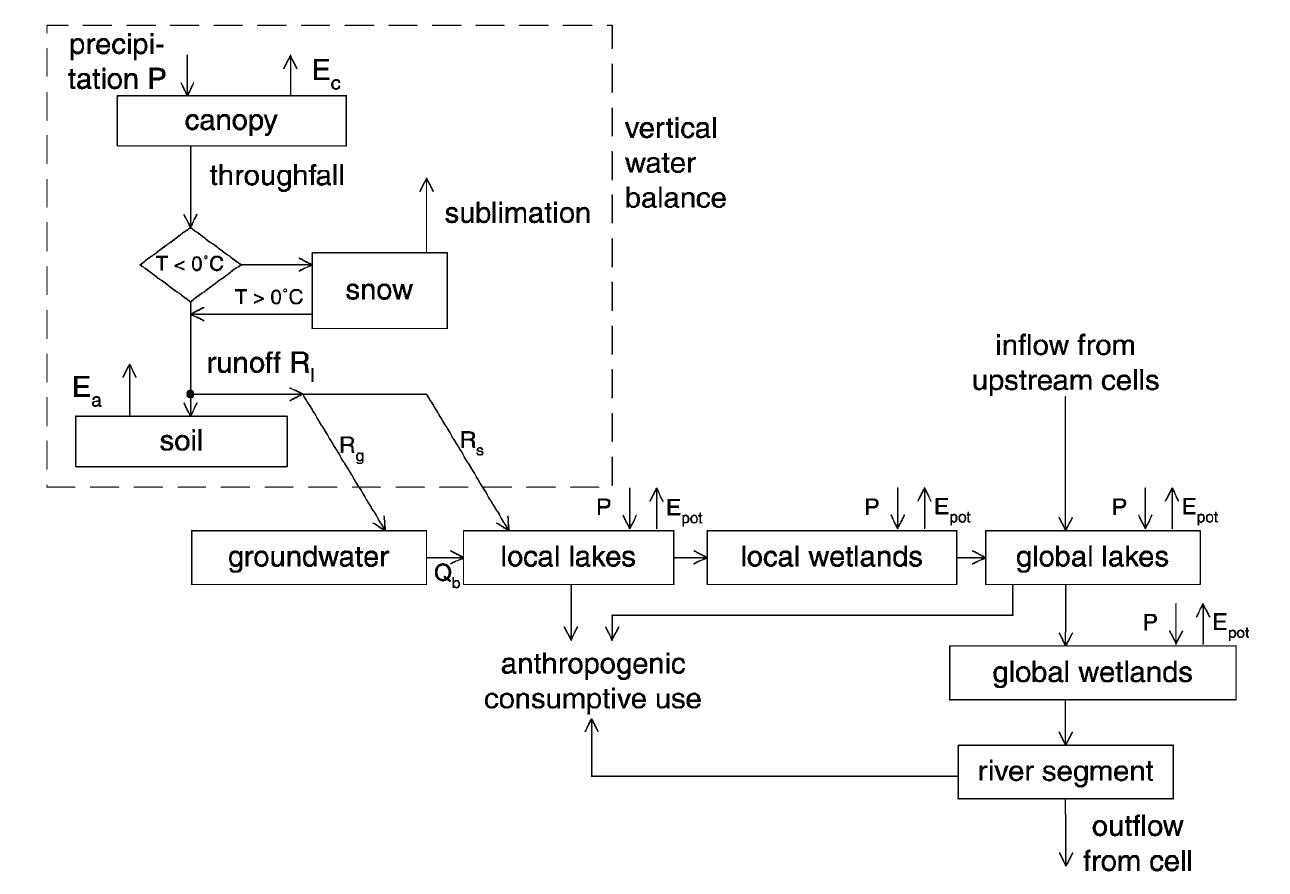
\includegraphics[width=15cm]{waterGAP.png}
\caption[Representation of a global hydrological from the WaterGAP software]{Representation of a global hydrological from the WaterGAP software \cite{doll}}
\label{waterGAP}
\end{figure}
Other runoff models exist, for example the WEAP model of the Stockholm Environment Institute \cite{weap}, the HYPE model developed by the Swedish Meteorological and Hydrological Institute \cite{hype}, or the TOPKAPI model of PROGEA \cite{topkapi}. \newline
Given that this work is part of the openFRED project (see Ch. \ref{chap:introduction}), the runoff data should eventually be accessible from open source databases or software. The weather aspects of the openFRED project are handled together with the Helmholtz Zentrum Geesthacht : the weather model COSMO is being adapted the the requirements of the project, and, when ready, will deliver the input data (rainfall, temperature, ...) for an existing open source runoff model. \newline
In the meantime, modeled time series from the WaterGAP software were used in this work. The data takes the form of a raster with a resolution of 5 angular minutes, each raster cell containing time series of runoff with a daily temporal resolution, from 2006 to 2009. When only the cells with an average runoff over \unit[100]{m\textsuperscript{3}\textperiodcentered s\textsuperscript{-1}} are displayed, the German river system is recognizable and the cells overlap the layout of Germany main rivers from the Digital Landscape Model \cite{dlm250} (see Fig. \ref{map_watergap_dlm}).

\begin{figure}[H]
\centering
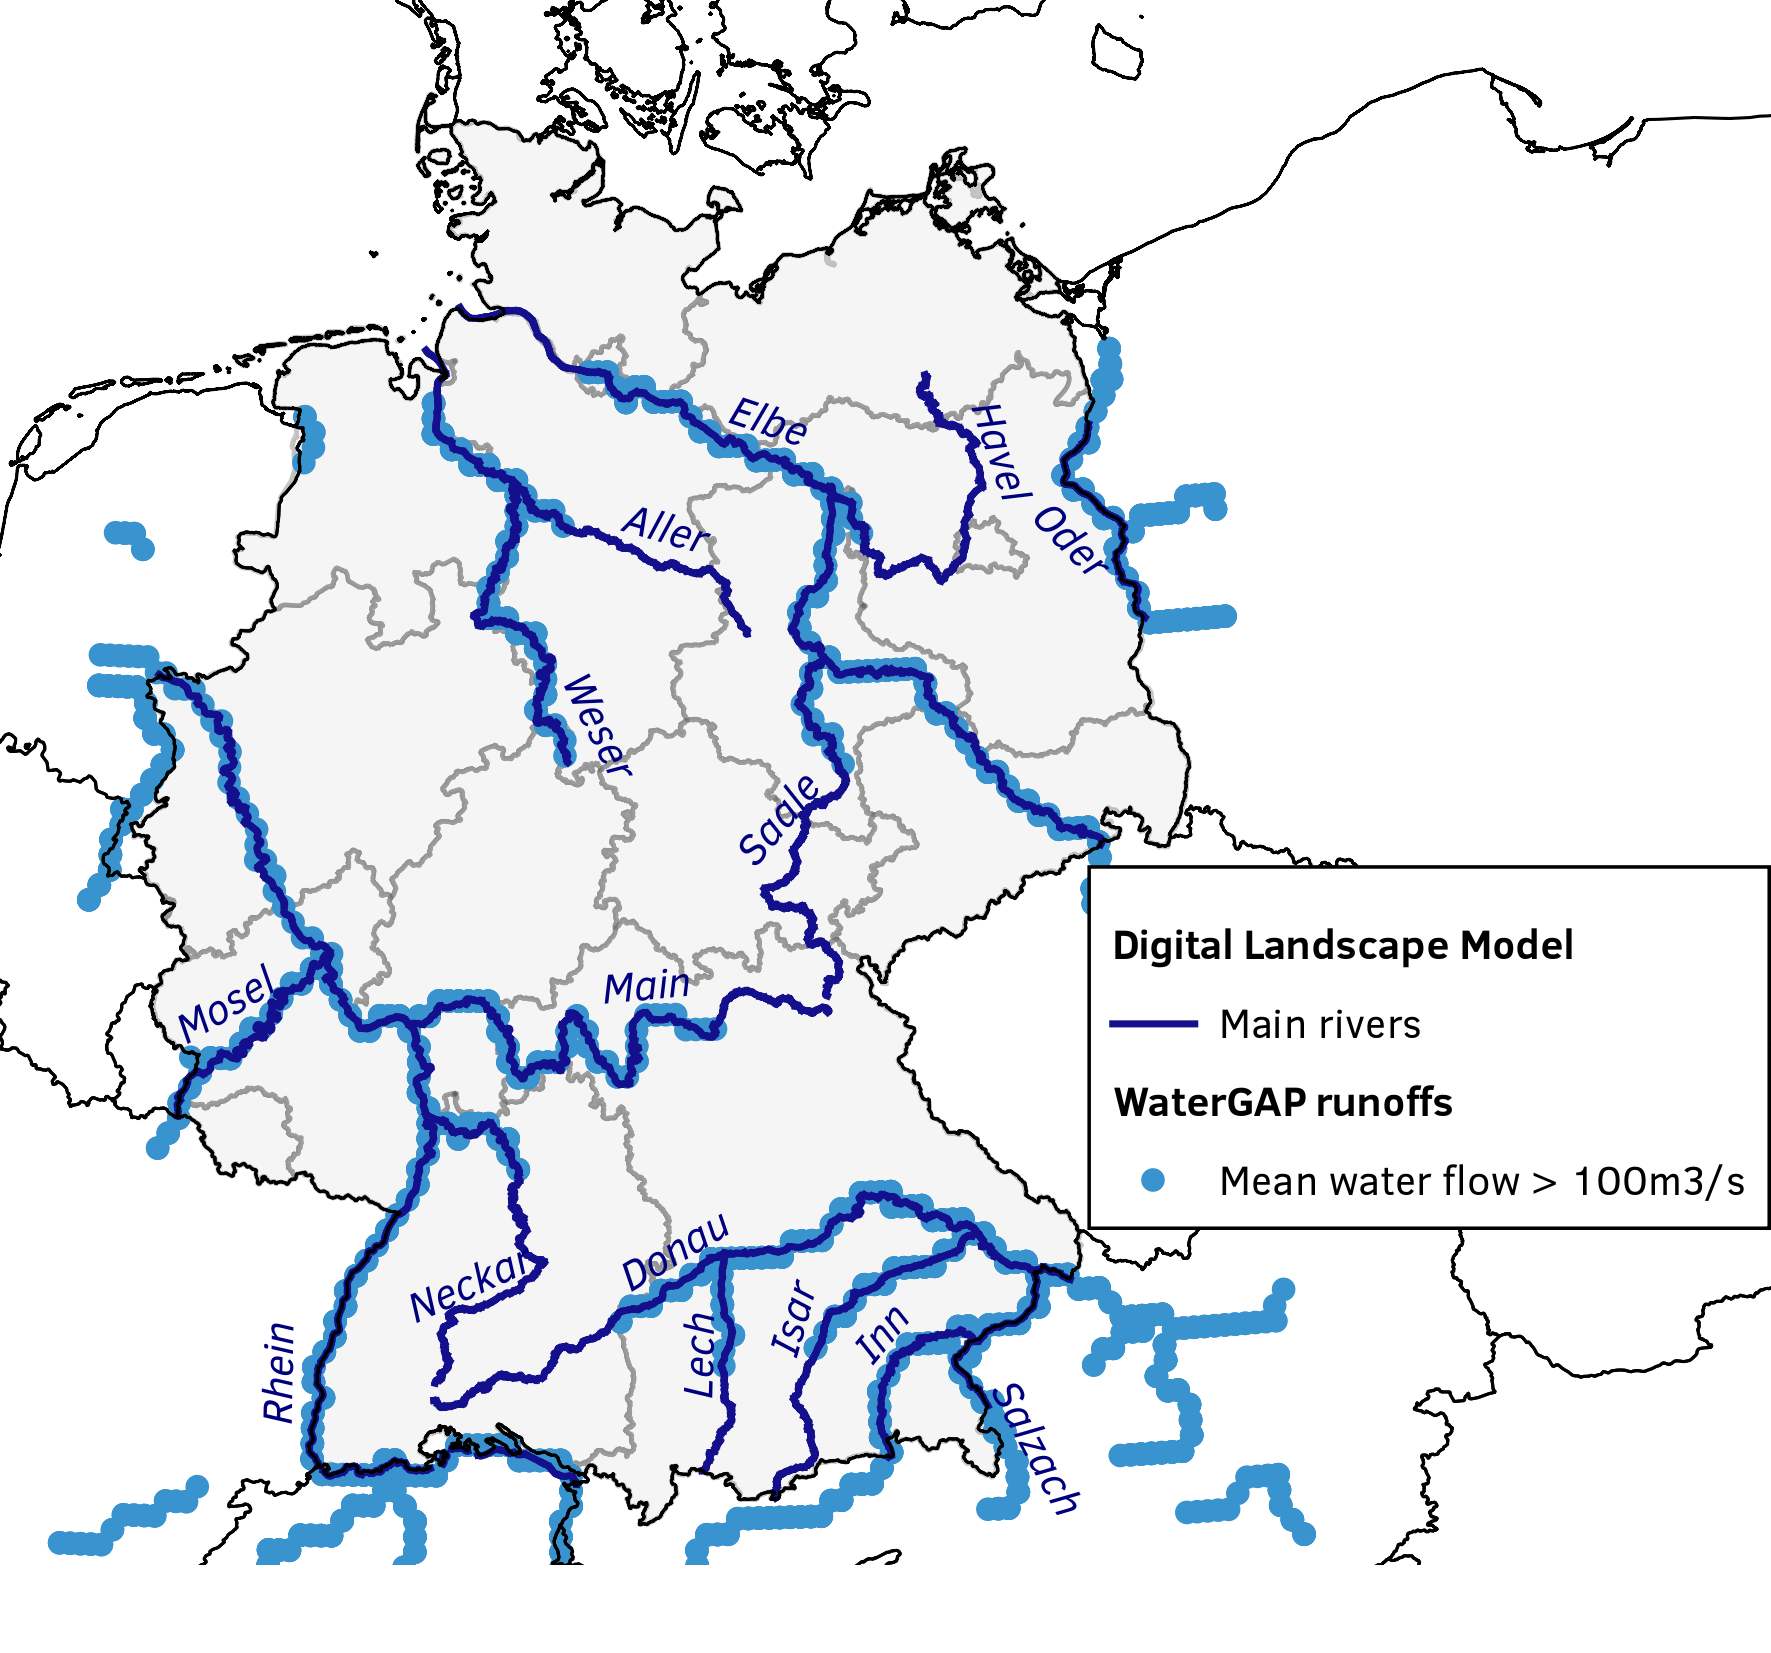
\includegraphics[width=13cm]{map_watergap_dlm.png}
\caption[Representation of the German main rivers from waterGAP and DLM]{Representation of the German main rivers from waterGAP and DLM}
\label{map_watergap_dlm}
\end{figure}
